\documentclass[15pt]{scrartcl}
\usepackage[sexy]{evan}
\newcommand{\R}{\mathbb{R}}
\newcommand{\N}{\mathbb{N}}
\newcommand{\Q}{\mathbb{Q}}
\newcommand{\Z}{\mathbb{Z}}
\newcommand{\F}{\mathbb{F}}
\usepackage{relsize}
\setcounter{secnumdepth}{0}
\begin{document}
\title{A Companion to Aluffi's Algebra Chapter 0}
\date{\today}
\author{Jiawen Huang}

\maketitle


    

\section{Acknowledgment}
\begin{enumerate}
    \item Thank Professor Paolo Aluffi for writing such a wonderful \href{https://bookstore.ams.org/gsm-104}{book}. 
    \item Main contributors of Discord Discussion Forum: \[\Large{\textbf{Arthur, Evie and Jiawen Huang (AB-BOY)}}\] (I don't know their real names). Thank Arthur and Evie for discussing many problems with me and helping me understand the book better. I would not be able to finish this companion without their help. 
    \item Thank Evan Chen for creating such a beautiful latex style. 
    \item English is not my first language. I apologize for any grammatical errors in this companion (in fact, a lot). Just ignore them. Not that deep. 
    \item This companion contains my personal notes, results I found beautiful and solutions to most of the challenging exercises. They may not be the best solutions or the most elegant ones. Please feel free to contact me if you have better solutions or suggestions. The discussions in chapter 1 and 2 are sort of meaningless and naive, but I included them for completion. 
    \item Algebra Chapter 0 is not as difficult as Lang's Algebra. So this companion is not necessary. But I hope it can help some readers who are new to abstract algebra or new to college-level math. 
    \item By the time I wrote this companion, I am a first year undergraduate student. There may be some mistakes in this companion. Please feel free to contact me if you find any mistakes or have any suggestions. 
    \begin{center}
        My website: https://amazingboboy.github.io/my-website/.
        \\
        My email: kevin47900 [at] gmail [dot] com
    \end{center}
\end{enumerate}
\section{Recommendations for readers}
\begin{itemize}
    \item Do not skip any word in the first seven chapters, read it word by word. Aluffi is a gifted writer. 
    \item Please do all the exercises if you are new to abstract algebra. And that was what I did when I was reading the book for the first time. This is important because abstract algebra is very different from other branches of math you may have seen before. It's a language that you need to get used to. Also, there are a lot of interesting results hidden in the exercises, especially in the later chapters! My favorites are the series of exercises about the norm and trace functions in chapter 7. At the end, Aluffi introduces Hilbert's Theorem 90 as an application. This is really cool! (So Hilbert's Theorem 90 basically gives you all the rational solution to Pell's equation if you have learned about it in math competitions before).
    \item This is a book famous for its early introduction to category theory. But in fact, this book has a lot of other advantages: great exercises, hint, Internal references if you are using pdf version, etc.  You will find out as you read more. If one day there is an Algebra chapter 1 by Aluffi, I will be the first to buy it.
\end{itemize}

\newpage 
\tableofcontents
\newpage
\section{Chapter 1: Preliminaries}
This chapter is mainly a review of basic concepts in set theory and category theory. My recommendations for readers: 
\begin{itemize}
    \item Do not skip this chapter, read it word by word. Aluffi is a gifted writer. JUST BE PATIENT and READ. There are many subtle details that you probably have not seen before. 
    \item Try to do all the exercises. Most exercises are straightforward and don't take too much time but really help you solidify the concepts. This is especially important for readers who have not seen category theory before.
    \item The most important information (in my opinion) you need to take away from this chapter is the universal property. You may think it's useless at first, but I promise it will make sense once you get to section 7 of chapter 2. 
    \item Don't feel bad if you don't feel like you fully understand category theory after reading this chapter. This is normal. It's indeed abstract nonsense if you have no context to apply it to. The problem that makes me realize the power and clarity of category theory is Exercise 7.12 from chapter 2 (prove $F^{ab}(A)\cong F/[F,F]$). You may want to take a look at it when you get there. 
    \item Good Luck!
\subsection{Exercise }
\begin{discussion*}Exercise 
    \begin{abboy*}
    
    \end{abboy*}
    \begin{arthur*}
    
    \end{arthur*}
    \begin{evie*}
    
    \end{evie*}
\end{discussion*}

\subsection{Exercise 2.5}
\begin{discussion*}Formulate a notion of epimorphism, in the style of the notion of monomorphism seen in §2.6, and prove a result analogous to Proposition 2.3, for epimorphisms and surjection. 
    \begin{abboy*}
    If f is an epimorphism, then f is surjective. 
    \\
    Not easy. 
    \\
Its form: for all sets Z and all functions $a'$ and $a'': B\to Z$, if $a'f=a''f$, then $a'=''a$. 
\\
Proof: $f: A\to B$. Assume f is not surjective for the sake of contradiction, then  there msut exist $b_0$ such that $b_0$ is not in $Im(f)$. Construct $a'(b_0)=1$ and $a''(b_0)=2$, and $a'(Im(f))=a''(Im(f))$ then $a'f=a''f$ but $a'$ doesn't equal to $a''$. Contradiction!
    \end{abboy*}

\end{discussion*}
\subsection{Exercise 4.4}

\begin{discussion*}Exercise 4.4
    \begin{abboy*}
    For second question, how can you have a category $C_{nonmono}$ without monomorphism? It must have identity right?
    \end{abboy*}
    \begin{abboy*}
    btw any two non-monomorphism composition will be non-monomorphism. 
    \end{abboy*}
    \begin{arthur*}
    yeah, you can't have such a category, because the identity is always a monomorphism.
    \end{arthur*}
\end{discussion*}
\subsection{Exercise 5.9}

\begin{discussion*}Exercise 5.9
    \begin{abboy*}
    Say $A$, $B$ and $C$ are objects in category $\textbf{C}$. I think $A \times B \times C$ doesn't make sense in most category. In $SET$, it makes snese becasue $A\times B$ is also a set. But in general, $A \times B$ may not be the object of $\textbf{C}$. Then $(A\times B) \times C$ doesn't make sense.
    \end{abboy*}
    \begin{abboy*}
    $@$Evie
    \\

product of objects doesn't amke sense soemtimes
    \end{abboy*}
    \begin{evie*}
    "category with products" means a category where any two (or more, including infintely many) objects have a product in the category
    \begin{center}
        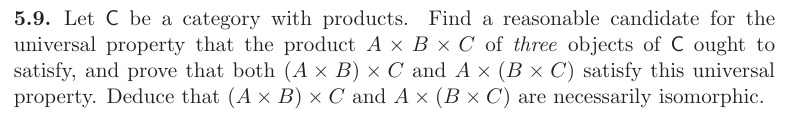
\includegraphics[scale=0.6]{pic1.png}
    \end{center}
    \end{evie*}
\end{discussion*}
\end{itemize}
\section{Chapter 2: Groups, first encounter}
If you have time, please try Exercise 7.12. 

\end{document}